\documentclass[10pt,oneside]{mwbk}

% ustawienia kodowania pliku i języka
\usepackage[T1]{polski}
\usepackage[utf8]{inputenc}

\usepackage{indentfirst}
\usepackage{graphicx}


% czcionka Times
\usepackage{times}

% odstępy na 1.5 (pomimo, iż linespread jest na 1.3
\linespread{1.3}

% dzielenie wyrazów – większe odstępy, mniej dzielenia
\hyphenpenalty=5000
\tolerance=5000

%import z pliku csv
\usepackage{csvsimple}

%strona tytułowa
\renewcommand {\maketitle}{
\begin {titlepage}
\begin {center}
	\LARGE
	\textbf {PROJEKTOWANIE ALGORYTMOW I METODY SZTUCZNEJ INTELIGENCJI}
	\newline
	\newline
	\textit {SPRAWOZDANIE Z  LABORATORIUM}
	\textbf{ Tablica asocjacyjna}
	\newline
	\begin{table}
	\begin{center}
	\begin{tabular}{rl}
	IMIĘ I NAZWISKO & Mariusz Dajczak \\
	NR INDEKSU & 200403 \\	
	TERMIN & czwartek 10:00-12:35 \\
	DATA  & 27.03.2014 \\
	\end{tabular}

	\end{center}
	\end{table}
\end {center}
\end {titlepage}}

\renewcommand*\thesection{\arabic{section}} % zmiana numeracji sekcji 0.X -> X
\begin{document}
\maketitle
\section{Wstęp}
	

	\indent Tablica asocjacyjna to abstrakcyjny typ danych, który przechowuje pary elementów: klucz i wartość. Ten obiekt jest również nazywany słownikiem lub mapą. W bibliotekach C++ istnieje szablon std::map, który jest implementacją tablicy asocjacyjnej. \\
	\indent Celem tego ćwiczenia było zaimplementowanie tablicy asocjacyjnej na 3 różnych strukturach danych:
	\begin {itemize}
		\item        lista z STL,
		\item  binarne drzewo poszukiwań,
		\item  tablica haszująca z funkcją mieszającą.\\
	\end {itemize} 
	Następnie należało przetestować czas dostępu do elementu dla różnych implementacji.
\section {Wyniki pomiarów}
	\subsection {Binarne drzewo poszukiwań}

	\begin{table}[h]
	\centering
    \begin{tabular}{|l|l|}
    \hline
     Rozmiar problemu & Czas wykonania \\ \hline
    10                & 18.5           \\ \hline
    100               & 20.9           \\ \hline
    1000              & 21.9           \\ \hline
    10000             & 20.1           \\ \hline
    100000            & 18             \\ \hline
    1000000           & 20.4           \\ \hline
    10000000          & 21.3           \\ \hline
    \end{tabular}
    \caption {Pomiary czasu dla implementacji na BST}
\end{table}

	\subsection {Tablica haszująca}
	
	\begin{table}[h]
	\centering
    \begin{tabular}{|l|l|}
    \hline
     Rozmiar problemu & Czas wykonania \\ \hline
    10                & 22.1           \\ \hline
    100               & 21.1           \\ \hline
    1000              & 25.8           \\ \hline
    10000             & 56.1           \\ \hline
    100000            & 475.9          \\ \hline
    1000000           & 4074.8         \\ \hline
    10000000          & 52219.1        \\ \hline
    \end{tabular}
    \caption {Pomiary czasu dla implementacji na tablicy haszującej}
\end{table}
	
	\newpage
	\section { Zestawienie}
	Na wykres naniosłem 2 funkcje odniesienia:
	\begin {itemize}
		\item        $f(n)=n$ - kolor czarny
		\item  $f(n)=logn$ - kolor fioletowy\\
	\end {itemize} 
	
	\begin{figure}[!h]
	\centering
	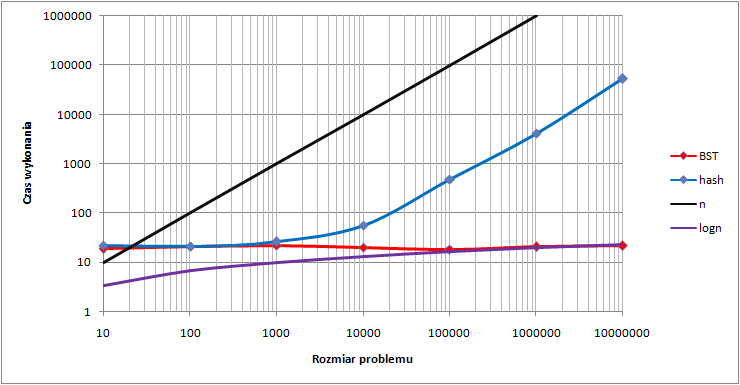
\includegraphics[scale=0.8]{wykres.png}
	\caption{ Złożoność obliczeniowa dostępu do elementu}
	\end{figure}
	
\section {Wnioski}
\indent Po przeprowadzeniu symulacji widzimy, że dla małego rozmiaru danych wejściowych czas dostepu do elementu jest identyczny dla obydwu implementacji.
Wraz z wzrostem rozmiaru problemu widoczna zaczyna być przewaga tablicy opartej na binarnym drzewie poszukiwań, której złożoność obliczniowa wynosi $logn$. W tablicy haszującej zaczynają powstawać kolizje, ponieważ elementów jest więcej niż rozmiar tablicy, i pod jednym jej indeksem znajduje się wiele kluczy (pod każdym indeksem znajduje się lista).
W takim przypadku algorytm przeszukuje liniowo owe listy i w efekcie złożoność czasowa wzrasta do liniowej. \\
\indent Implementacji na zwykłej liście nie udało mi się przetestować. Podczas próbnych testów na kontrolowanych danych wejściowych wszystko działało prawidłowo. Natomiast podczas testowania złożoności obliczeniowej dla wiekszych losowych danych program zawieszał się.
Co najlepsze moment , w którym przestawał działać był uzależniony od danych wejściowych i dla każdego  nowo wygenerowanego zestawu wysypywał się w innym momencie.

\end{document}